% https://www.youtube.com/watch?v=3yHAu8dPxVk&list=PLa_2246N48_rk8nzKg6VDykSEU6svwv4r&index=3

\documentclass{beamer}
\usetheme{Frankfurt}
\setbeamercovered{transparent}
\usepackage[utf8]{inputenc}

\title{Titulo}
\subtitle{Subtitulo}
\author[A.]{Autor}
\date{Data}
\institute[Inst.]{Intituição}
\logo{Imagem de logo}

\begin{document}

\begin{frame}
	\titlepage
\end{frame}

\begin{frame}
	\frametitle{Título Quadro 1}
	\framesubtitle{Subtitulo quadro 1}
	
	\begin{itemize}
		\item<1-> Slide 1
		\item<2-> Slide 2
		\item<3-> Slide 3
		\item<4-> Slide 4
	\end{itemize}
	
	\hypertarget<2>{segundo-slide-quadro1}{}
	\hyperlink{segundo-slide-quadro1}{Segundo slide com target no mesmo quadro}
	
	\hyperlink{terceiro-slide-quadro2}{Terceiro slide com target em outro quadro}
	
\end{frame}

\begin{frame}
	\frametitle{Título Quadro 2}
	\framesubtitle{Subtitulo quadro 2}
	
	\begin{itemize}
		\item<1-> Slide 1
		\item<2-> Slide 2
		\item<3-> Slide 3
		\item<4-> Slide 4
	\end{itemize}
	
	\hypertarget<3>{terceiro-slide-quadro2}{}
	
	\hyperlink{terceiro-quadro<4>}{Slide 4 do Quadro 3 usando label}
\end{frame}

\begin{frame}[label=terceiro-quadro] 
	\frametitle{Título Quadro 3}
	\framesubtitle{Usar label dispensa o uso do hypertarget}
	
	\begin{itemize}
		\item<1-> Slide 1
		\item<2-> Slide 2
		\item<3-> Slide 3
		\item<4-> Slide 4
	\end{itemize}

\end{frame}

\begin{frame}
	\frametitle{Título Quadro 4}
	\framesubtitle{Usando botões}
	
	\begin{itemize}
		\item<1-> Slide 1
		\item<2-> Slide 2
		\item<3-> Slide 3
		\item<4-> Slide 4
	\end{itemize}
	
		\hyperlink{segundo-slide-quadro1}{\beamerbutton{Segundo slide do quadro 1}}
		
		\hyperlink{segundo-slide-quadro1}{\beamergotobutton{Segundo slide do quadro 1}}
		
		\hyperlink{segundo-slide-quadro1}{\beamerskipbutton{Segundo slide do quadro 1}}
		
		\hyperlink{segundo-slide-quadro1}{\beamerreturnbutton{Segundo slide do quadro 1}}
		
\end{frame}

\begin{frame}
	\frametitle{Título Quadro 5}
	\framesubtitle{Destinos padrão do BEAMER}
	
	\begin{itemize}
		\item<1-> Slide 1
		\item<2-> Slide 2
		\item<3-> Slide 3
		\item<4-> Slide 4
	\end{itemize}
	
	\hyperlinkslidenext{Próximo Slide}
	
	\hyperlinkslideprev{Slide Anterior}
	
	\hyperlinkframestart{Início do quadro atual}
	
	% \hyperlinkappendixstart{Início do Apendice}
	
	% \hyperlinkappendixend{Fim do Apendice}
	
	\hyperlinkframeend{Final do Quadro atual}
	
	\hyperlinkframestartnext{Início do próximo Quadro}
	
	\hyperlinkframeendprev{Fim do Quadro Anterior}
	
	\hyperlinkpresentationstart{Início da apresentação}
	
	\hyperlinkpresentationend{Fim da apresentação}	
	
	
\end{frame}

\begin{frame}
\frametitle{Título Quadro 6}
\framesubtitle{Zoom em uma porção clicável da área do quadro}

\hypersetup{linkbordercolor=yellow}

%\framezoom<slide do link><slide onde aparece o zoom>(x_inicial, y_inicial)(largura, altura) --- eixo y é de cima para baixo
\framezoom<2><3>[border](3.5cm, 2.75cm)(2.5cm, 1cm)
\framezoom<2><4>[border=4](6cm, 2.75cm)(2.5cm, 1cm)
\begin{figure}
	\centering
	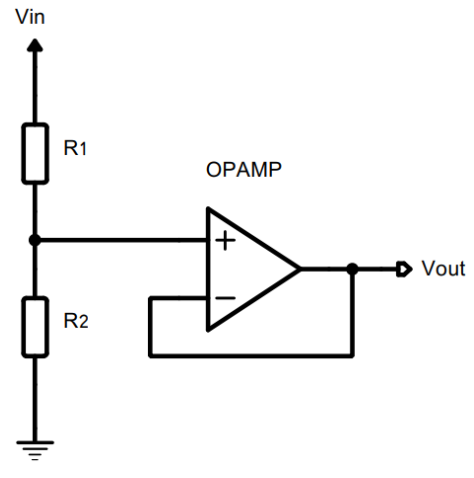
\includegraphics[scale=0.3]{figuras/divisorTensao_20241001b.png}
\end{figure}
	
\end{frame}

\end{document}